% LaTeX source for ``การเรียนรู้ของเครื่องสำหรับเคมีควอนตัม (Machine Learning for Quantum Chemistry)''
% Copyright (c) 2022 รังสิมันต์ เกษแก้ว (Rangsiman Ketkaew).

% License: Creative Commons Attribution-NonCommercial-NoDerivatives 4.0 International (CC BY-NC-ND 4.0)
% https://creativecommons.org/licenses/by-nc-nd/4.0/

\chapter{โมเดลการเรียนรู้ของเครื่องสำหรับเคมีควอนตัม}
\label{ch:chem_ml}

%--------------------------
\section{ANI-1}
\idxen{Model for Quantum Chemistry!ANI-1}
%--------------------------

ANI เป็นชื่อย่อสั้น ๆ ของโมเดล ANAKIN-ME ซึ่งย่อมาจาก Accurate NeurAl networK engINe for Molecular Energies อีกทีหนึ่ง 
โดยโมเดลตัวนี้ถูกพัฒนาด้วย Neural Network สำหรับการทำนายค่าพลังงานศักย์ของโมเลกุลโดยที่มีความแม่นยำในระดับเดียวกับการคำนวณด้วยวิธี 
DFT\autocite{smith2017a}

%--------------------------
\section{SchNet และ SchNOrb}
%--------------------------

%--------------------------
\subsection{SchNet}
\idxen{Model for Quantum Chemistry!SchNet}
%--------------------------

\autocite{schutt2017,schutt2018}

%--------------------------
\subsection{SchNOrb}
\idxen{Model for Quantum Chemistry!SchNOrb}
%--------------------------

SchNOrb ย่อมาจาก \enquote{SchNet for Orbitals}\autocite{schutt2019a}

%--------------------------
\section{GDML และ sGDML}
%--------------------------

%--------------------------
\subsection{GDML}
\idxen{Model for Quantum Chemistry!GDML}
%--------------------------

\autocite{chmiela2017}

%--------------------------
\subsection{sGDML}
\idxen{Model for Quantum Chemistry!sGDML}
%--------------------------

\autocite{chmiela2018}

\autocite{sauceda2020}

%--------------------------
\section{$\Delta$ML}
\idxen{Model for Quantum Chemistry!$\Delta$ML}
%--------------------------

งานวิจัยที่ใช้ Correction หรือผลต่างของผลลัพธ์จากการคำนวณและค่าอ้างอิงมาช่วยทำให้การทำนายคุณสมบัติของโมเลกุลมีค่าแม่นยำมากยิ่งขึ้นนั้น%
นั้นมีมานานแล้ว\autocite{hu2003,wu2007,balabin2009}

Delta-ML ($\Delta$ML) เป็นเทคนิคที่ใช้ค่าความแตกต่างระหว่างค่าอ้างอิง (Reference หรือจะเรียก Label ก็ได้) จากวิธีการคำนวณที่มีความ%
แม่นยำต่ำกับความแม่นยำสูงมาใช้ในการเทรนโมเดล (จึงเป็นที่มาว่าทำไมถึงเรียกว่า Detla) ซึ่งการทำแบบนี้จะช่วยให้โมเดลสามารถเรียนรู้การเชื่อมโยง 
(Transferability) ไปยังค่าที่ต้องการทำนายได้อย่างถูกต้องและแม่นยำมากขึ้น โดยจะมีความถูกต้องเทียบเคียงกับการใช้วิธีแบบดั้งเดิมที่มีความแม่นยำสูง 
(เช่น Post-HF) ตัวอย่างของการใช้ $\Delta$ML คือการใช้ค่าความแตกต่างของพลังงานที่ได้จากการคำนวณด้วยวิธี DFT และ CCSD(T) 
($y_{\text{DFT}} - y_{\text{CCSD(T)}}$) มาฝึกสอนโมเดล\autocite{ramakrishnan2015a}

จริง ๆ แล้ว $\Delta$ML ก็เป็นเทคนิคอันนึงที่มีแนวคิดมาจากความพยายามที่ต้องการจะทำให้โมเดลสามารถเรียนรู้ได้จากค่าความผิดพลาด (Error) 
โดยเริ่มมีการเอามาใช้กันมากขึ้นในช่วงปีที่ผ่านมา (ในช่วงแรกถูกใช้เยอะแค่ในเฉพาะกลุ่มวิจัยในโซนยุโรป สำหรับการเอามาทำนายพลังงานและ%
เกรเดียนต์ของพลังงาน (Energy Gradient) ซึ่งก็สอดคล้องกับแรงของแต่ละอะตอมในโมเลกุลโมเลกุลนั่นเอง

%--------------------------
\section{Graph Neural Network}
\idxth{โครงข่ายประสาทแบบกราฟ}
\idxen{Graph Neural Network}
%--------------------------

โครงข่ายประสาทแบบกราฟ (Graph Neural Network หรือ GNN) เป็นโครงข่ายประสามแบบหนึ่งซึ่งจะมองความสัมพันธ์ภายในโครงสร้างข้อมูลให้%
อยู่ในรูปแบบของกราฟแบบ 2 มิติ โดยไอเดียนี้ได้ถูกเสนอตั้งแต่ปี ค.ศ. 2008\autocite{scarselli2009,zhou2020}

%--------------------------
\subsection{Message Passing Neural Network}
\idxth{โครงข่ายประสาทแบบการส่งข้อความ}
\idxen{Message Passing Neural Network}
%--------------------------

โครงข่ายประสาทแบบการส่งข้อความ (Message Passing Neural Network หรือ MPNN) เป็น GNN ประเภทหนึ่งซึ่งถูกนำเสนอครั้งแรกเมื่อปี 
ค.ศ. 2017\autocite{gilmer2017}

\begin{figure}[H]
    \centering
    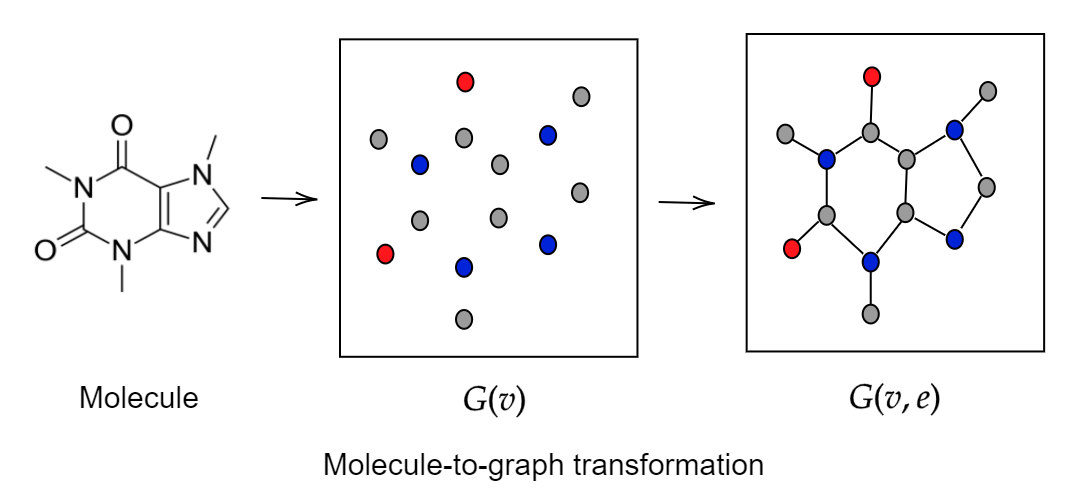
\includegraphics[width=\linewidth]{fig/mol-2-graph.png}
    \caption{การแทนโมเลกุลด้วยกราฟ}
    \label{fig:mol_2_graph}
\end{figure}

\begin{figure}[H]
    \centering
    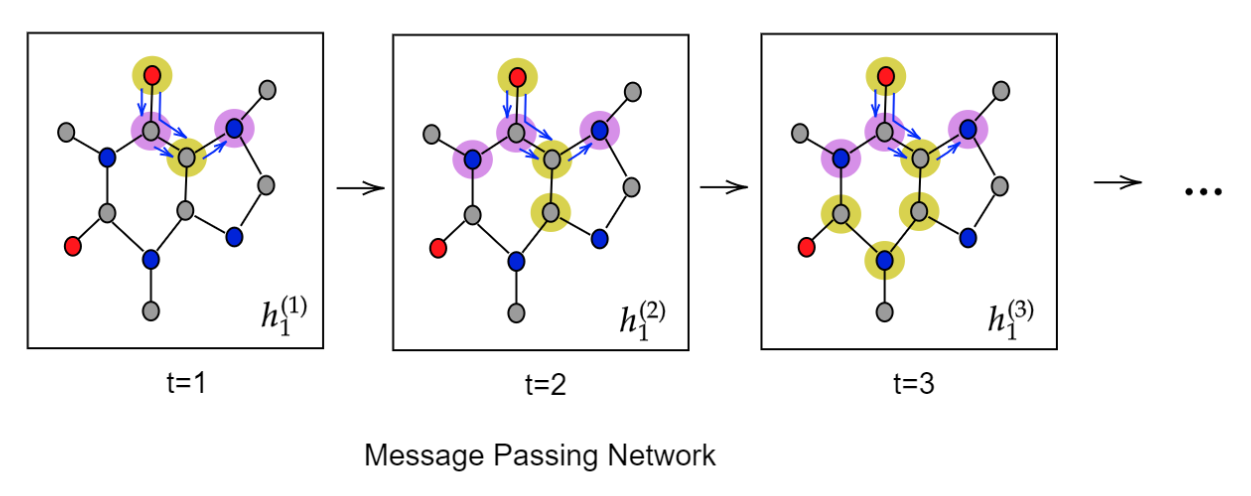
\includegraphics[width=\linewidth]{fig/mp-network.png}
    \caption{โครงข่ายของการส่งข้อความ}
    \label{fig:mp_network}
\end{figure}

\begin{figure}[H]
    \centering
    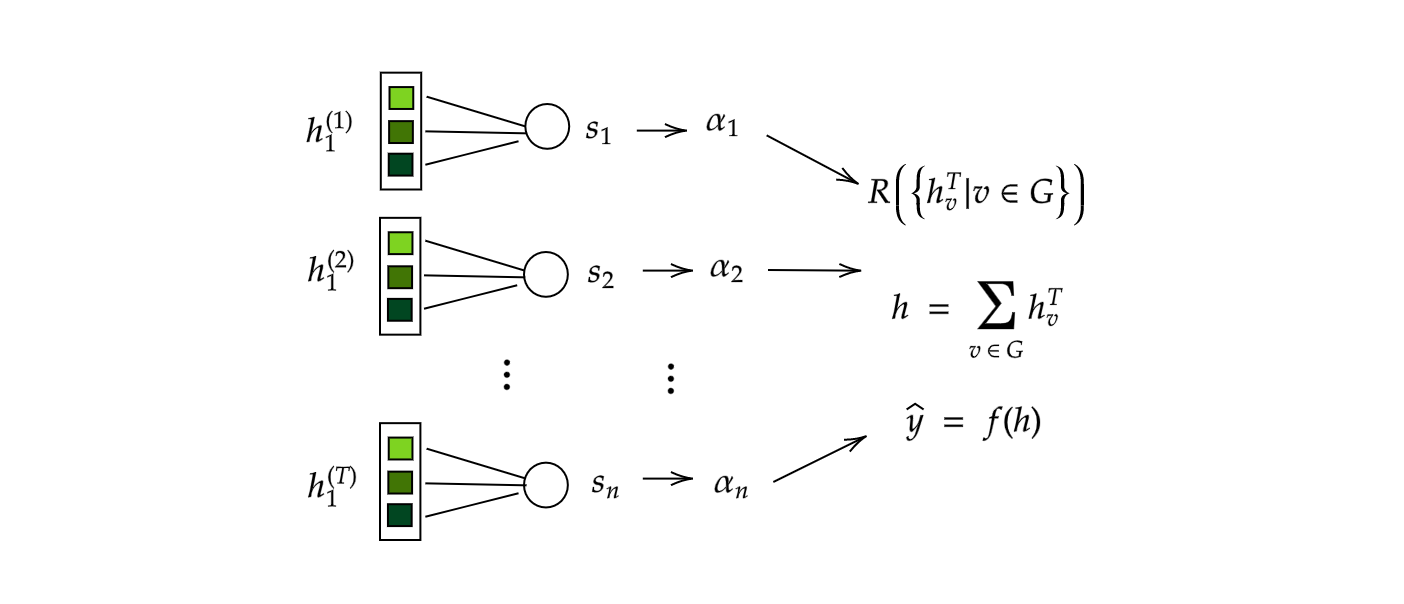
\includegraphics[width=\linewidth]{fig/mp-operation.png}
    \caption{การดำเนินการของการส่งข้อความ}
    \label{fig:mp_operation}
\end{figure}

%--------------------------
\section{Molecule Attention Transformer}
\idxth{ตัวแปลงความสนใจเชิงโมเลกุล}
\idxen{Molecule Attention Transformer}
%--------------------------
